Alle Messungen werden mit einem x-y-Schreiber aufgezeichnet. Die Graphen, die dieser Auswertung zu Grunde liegen, sind im Anhang~\ref{sec:anhang} zu sehen.
Messung 1 (Abb.~\ref{fig:messung1})  und Messung 2 (Abb.~\ref{fig:messung2}) gehen in Kapitel~\ref{sec:auswertung1} ein, wobei Messung 1 zusätzlich in Kapitel~\ref{sec:auswertung4} verwendet wird. Messung 3 (Abb.~\ref{fig:messung3})-- die Frank-Hertz-Kurve --  wird im Auswertungsteil~\ref{sec:auswertung3} analysiert. Messung 4 (Abb.~\ref{fig:messung4})wird in Kapitel~\ref{sec:auswertung4}
 benötigt.
\subsection{Statistische Formeln}
\subsubsection{Fehlerrechnung}
\label{sec:Fehlerrechnung}
Im folgenden wurden Mittelwerte von $N$ Messungen der Größe $x$ berechnet
\begin{equation}
\bar{x} =  \frac{1}{N} \sum_{i=1}^\text{N} x_i \ ,
\end{equation}
sowie die Varianz
\begin{equation}
V(x) = \frac{1}{N} \sum_{i=1}^\text{N} (x_i - \bar{x})^2
\end{equation}
woraus die Standardabweichung folgt
\begin {equation}
\sigma_x = \sqrt{V(x)}.
\end{equation}
Die Standardabweichung des Mittelwertes
\begin{equation}
\Delta_{x} = \frac{\sigma_x}{\sqrt{N}} \ ,
\end{equation}
kürzer auch Fehler des Mittelwertes genannt, bezieht noch die Anzahl der Messungen mit ein. \\
Liegen $N$ Messwerte $x_i$ mit Fehlern $\Delta_{x_i}$ vor, so wird aus ihnen ein gewichteter Mittelwert sowie ein gewichteter Fehler berechnet:
\begin{align}
	\bar{x} &= \frac{\sum_{i=1}^N \left(\frac{x_i}{\Delta_{x_i}^2} \right)}{\sum_{i=1}^N \left(\frac{1}{\Delta_{x_i}^2} \right)} \\
	\Delta_x &= \sqrt{\frac{1}{{\sum_{i=1}^N \left(\frac{1}{\Delta_{x_i}^2} \right)}}} \quad .
\end{align}
Des weiteren ist die Gaußsche Fehlerfortpflanzung definiert als
\begin{equation}
\Delta_A = \sqrt{ \sum_{i=1}^N  \left(   \frac{\partial A(x_1, ... ,x_N)}{\partial x_i} \right)^2 \Delta_{x_i} ^2 } \quad .
\end{equation}


\subsection{Anzahl der Stöße in der Röhre}
Für das Gelingen des Versuches ist es wichtig, dass weder zu viele noch zu wenige Elektronen mit Quecksilberatomen zusammenstoßen. Bei zu wenig Stößen treten kaum Wechselwirkungen auf, die beobachtet werden sollen. Gibt es hingegen zu viele Stöße, sind einige elastisch unter Änderung der Richtung, sodass sie nicht an der Kathode ankommen und fälschlicherweise nicht zu Strom beitragen. \\
Aus den Temperaturen in Kelvin lässt sich nach Gleichung \eqref{eq:weglange} und \eqref{eq:dampfdruck} der Sättigungsdruck und daraus die freie Weglänge d.h. die Strecke, die ein Teilchen ohne Kollisionen zurücklegt, berechnet. Die Ergebnisse sind in Tabelle \ref{tab:temperaturen} dargestellt.



\begin{figure}[h!]
	\centering
	\captionof{table}{Anzahl der Stöße in der \SI{1}{\centi\meter} langen Röhre}
	\begin{tabular}{cccc}
		Temperatur / \si{\kelvin} & Sättigungsdruck / \si{\milli\bar} & freie Weglänge / \si{\micro\meter} & Anzahl Stöße \\
		\hline
		298.15 & 0.01  & 5468.00 & 1.83    \\
413.15 & 3.25  & 8.91    & 1122.17 \\
453.15 & 14.14 & 2.05    & 4876.12 \\
373.15 & 0.55  & 53.06   & 188.48  \\

	\end{tabular}
	\label{tab:temperaturen}
\end{figure}




\subsection{Differentielle Energieverteilung} \label{sec:auswertung1}
Aus der Messung des Stromes bei veränderlicher Bremsspannung $U_A$ kann die Energieverteilung der austretenden Elektronen bestimmt werten
\begin{align}
	E(U_A) \sim \frac{I(U_A)-I(U_{A+1})}{U_A - U_{A+1}}
\end{align}

Strom und Spannung sind bekannt. Sie werden mit Hilfe eines x-y-Schreibers aufgenommen. Es werden zwei Messreihen für die Temperaturen T = \SI{25}{\celsius} und T = \SI{140}{\celsius} erstellt. Die Werte des Stromes für T = \SI{25}{\celsius} sind in Tabelle~\ref{tab:stromverlauf_25} zu finden und die Steigung  (Tabelle~\ref{tab:energieverteilung_25}) in Abbildung~\ref{fig:energieverteilung_25} grafisch dargestellt, während die Daten zu T = \SI{140}{\celsius} in den Tabellen~\ref{tab:stromverlauf_140} und~\ref{tab:energieverteilung_140} und der Abbildung~\ref{fig:energieverteilung_140}  stehen. \\
Aus der Energieverteilung bei Raumtemperatur kann das Kontaktpotential bestimmt werden (siehe Kapitel~\ref{cap:kontaktpotential} ).




\begin{figure}
	\centering
	\captionof{table}{Strom in Abhängigkeit der Spannung  (T = \SI{25}{\celsius})}
	\begin{tabular}{cc}
		Spannung / \si{\volt} & Strom /  \si{\nano\ampere}   \\
		\hline
		0.00 & 3800 \\
0.18 & 3747 \\
0.61 & 3614 \\
1.05 & 3561 \\
1.49 & 3401 \\
1.93 & 3269 \\
2.37 & 3136 \\
2.81 & 3003 \\
3.25 & 2870 \\
3.68 & 2750 \\
4.12 & 2617 \\
4.56 & 2471 \\
5.00 & 2338 \\
5.44 & 2166 \\
5.88 & 1993 \\
6.32 & 1807 \\
6.75 & 1608 \\
7.19 & 1382 \\
7.63 & 1116 \\
8.07 & 771  \\
8.29 & 531  \\
8.51 & 213  \\
8.73 & 53   \\
8.95 & 0    \\

	\end{tabular}
	\label{tab:stromverlauf_25}
\end{figure}

\begin{figure}
	\centering
	\captionof{table}{Steigung es Stromverlaufes (T = \SI{25}{\celsius}) und zugehörige Spannungswerte}
	\begin{tabular}{cc}
		Spannung / \si{\volt} & Strom pro Spannung / \si{\nano\ampere\per\volt}   \\
		\hline
		0.00 & 302.94  \\
0.18 & 302.94  \\
0.61 & 121.17  \\
1.05 & 363.52  \\
1.49 & 302.94  \\
1.93 & 302.94  \\
2.37 & 302.94  \\
2.81 & 302.94  \\
3.25 & 272.64  \\
3.68 & 302.94  \\
4.12 & 333.23  \\
4.56 & 302.94  \\
5.00 & 393.82  \\
5.44 & 393.82  \\
5.88 & 424.11  \\
6.32 & 454.41  \\
6.75 & 514.99  \\
7.19 & 605.87  \\
7.63 & 787.64  \\
8.07 & 1090.57 \\
8.29 & 1454.10 \\
8.51 & 727.05  \\
8.73 & 242.35  \\

	\end{tabular}
	\label{tab:energieverteilung_25}
\end{figure}


\begin{figure}
	\centering
	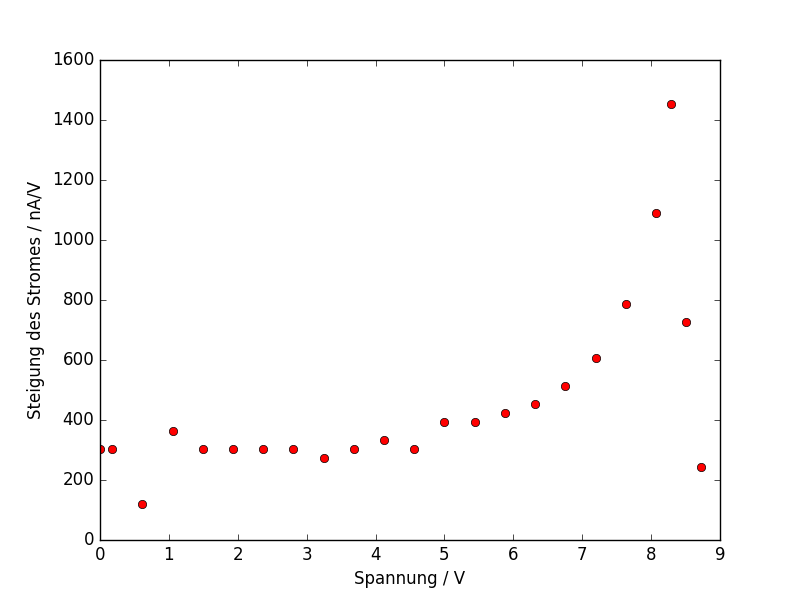
\includegraphics[width=0.9\textwidth]{build/Energieverteilung_25.png}
	\caption{Energieverteilung bei  T = \SI{25}{\celsius} ist proportional zur Steigung des Stromes}
	\label{fig:energieverteilung_25}
\end{figure}

\begin{figure}
	\centering
	\captionof{table}{Strom in Abhängigkeit der Spannung  (T = \SI{140}{\celsius})}
	\begin{tabular}{cc}
		Spannung / \si{\volt} & Strom /  \si{\nano\ampere}   \\
		\hline
		0.00 & 110 \\
0.22 & 97  \\
0.44 & 88  \\
0.66 & 81  \\
0.88 & 73  \\
1.11 & 65  \\
1.33 & 58  \\
1.55 & 51  \\
1.77 & 45  \\
1.99 & 38  \\
2.21 & 32  \\
2.43 & 26  \\
2.65 & 20  \\
2.88 & 15  \\
3.10 & 12  \\
3.32 & 9   \\
3.54 & 6   \\
3.76 & 4   \\
3.98 & 3   \\

	\end{tabular}
	\label{tab:stromverlauf_140}
\end{figure}

\begin{figure}
	\centering
	\captionof{table}{Steigung es Stromverlaufes (T = \SI{140}{\celsius}) und zugehörige Spannungswerte}
	\begin{tabular}{cc}
		Spannung / \si{\volt} & Strom pro Spannung / \si{\nano\ampere\per\volt}   \\
		\hline
		0.00 & 57.82 \\
0.22 & 40.48 \\
0.44 & 34.69 \\
0.66 & 34.69 \\
0.88 & 34.69 \\
1.11 & 34.69 \\
1.33 & 28.91 \\
1.55 & 28.91 \\
1.77 & 28.91 \\
1.99 & 28.91 \\
2.21 & 28.91 \\
2.43 & 23.13 \\
2.65 & 23.13 \\
2.88 & 17.35 \\
3.10 & 11.56 \\
3.32 & 11.56 \\
3.54 & 11.56 \\
3.76 & 5.78  \\

	\end{tabular}
	\label{tab:energieverteilung_140}
\end{figure}


\begin{figure}
	\centering
	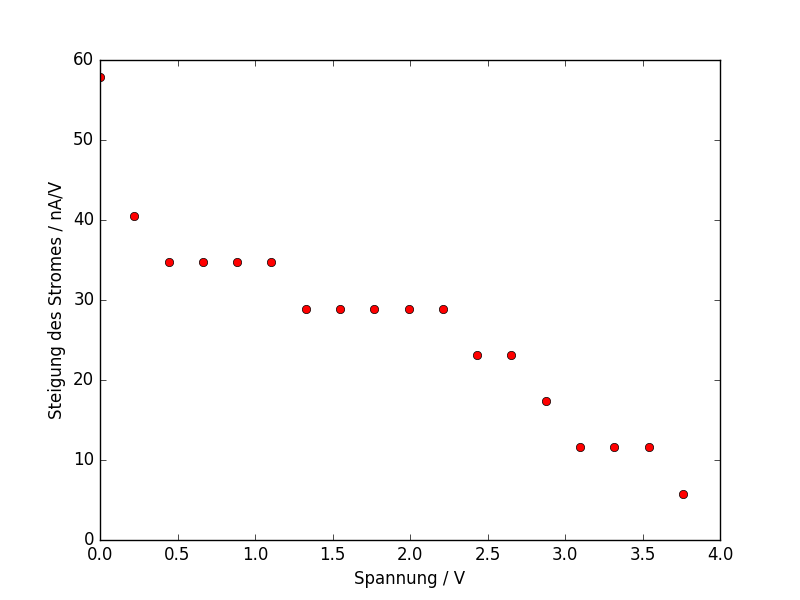
\includegraphics[width=0.9\textwidth]{build/Energieverteilung_140.png}
	\caption{Energieverteilung bei  T = \SI{140}{\celsius} ist proportional zur Steigung des Stromes}
	\label{fig:energieverteilung_140}
\end{figure}

\clearpage

\subsection{Erste Anregungsenergie des Quecksilberatoms}\label{sec:auswertung2}
Die erste Anregungsenergie wird aus den Abständen der Maxima der Frank-Hertz-Kurve bestimmt. Die Spannungsdifferenzen sind in Tabelle~\ref{tab:anregungsspannung} dargestellt. Ihr Mittelwert und deren Fehler ist

\begin{align}
	U_{\text{Mittel}} = \SI{4.95+-0.18}{\volt}
 \quad .
\end{align}

\begin{figure}[h!]
	\centering
	\captionof{table}{Die Differenzen der Strommaxima der Frank-Hertz-Kurve entsprechen der Anregungsspannung des Quecksilberatoms}
	\begin{tabular}{c}
		Spannung / \si{\volt}   \\
		\hline
		4.6216 \\
5.2297 \\
4.9865 \\

	\end{tabular}
	\label{tab:anregungsspannung}
\end{figure}

Aus der Anregungsspannung kann mit Hilfe den Formeln \eqref{eq:energie1} und \eqref{eq:energie2} die Anregungsenergie und daraus die Wellenlänge bestimmt werden.
Für die Anregungsenergie ergibt sich der Wert
\begin{align}
	\Delta E = \SI{7.92+-0.28e-19}{\joule}

\end{align}
und für die Wellenlänge 
\begin{align}
	\lambda = \begin{center}
\begin{tabular}{c}
	Wellenlänge $\lambda$ in mm \\
	\hline
	17.79 \\
	16.98 \\
	17.78 \\
	18.21 \\	
\end{tabular}
\captionof{table}{Wellenlänge}
\end{center} \quad .
\end{align}
Die Fehler werden jeweils mit Hilfe der Gaußschen Fehlerfortpflanzung berechnet
\begin{align}
	\sigma_{\Delta E} = \left|e_0 \sigma_{U_\text{Mittel}}\right|
\end{align}
und
\begin{align}
	\sigma_\lambda = \left|\frac{h c_0}{e_0} \frac{1}{U^2_{\text{Mittel}}} \sigma_{U_\text{Mittel}}\right| \quad .
\end{align} 



\subsubsection{Bestimmung der Kontaktpotentials} \label{sec:auswertung3}
\label{cap:kontaktpotential}
\underline{Methode 1:} \\
Die Frank-Hertz-Kurve ist genau um das Kontaktpotential $K$ nach rechts verschoben. Das erste Maximum liegt bei
\begin{align}
	U_1 = \SI{8.0256}{\volt} \quad .
\end{align}
Folglich ist das Kontaktpotential
\begin{align}
K_1 = U_1 - U_{\text{Mittel}} = \SI{3.08+-0.18}{\volt}
\end{align}
\underline{Methode 2:} \\
In Abbildung \ref{fig:energieverteilung_25} ist erkennbar, dass bei einer Bremsspannung $U_{A, \text{max}}$ von \SI{8.15}{\volt} Elektronen die größte Energie haben. Das Kontaktpotential ist die Differenz der Bremsspannung bei größter Energie und der konstanten Beschleunigungsspannung $U_B = \SI{11}{\volt} $.
\begin{align}
	K_2 = U_B - U_{A, \text{max}} =  \SI{2.85}{\volt} 
\end{align}

\subsubsection{Bestimmung der Ionisierungsspannung}\label{sec:auswertung4}
Die Ionisierungsspannung $U_\text{ION}$ ergibt sich aus der letzten Messung des Stromes bei einer höheren Gegenspannung von \SI{30}{\volt}. Um sie zu bestimmen wird eine möglichst steile Asymptote an den Stromverlauf angelegt. Die Beschleunigungsspannung, bei der diese Asymptote die Spannungsachse schneidet ist
\begin{align}
	U'_1 = \SI{13}{\volt} \ .
\end{align}
Sie setzt sich zusammen aus der Ionisierungsspannung und dem Kontaktpotential $K$, wobei für K der Mittelwert der in Kapitel \ref{cap:kontaktpotential} bestimmten Werte $K_1$ und $K_2$
\begin{align}
	K = \frac{K_1+K_2}{2} = \SI{2.965}{\volt}
\end{align}
angenommen wird. 
\begin{align}
	U_\text{ION} = U'_1 - K = \SI{10.035}{\volt}
\end{align}